\chapter{绪论}

\section{研究背景及意义}
\label{sec:1.1}

自2022年末,OpenAI推出的ChatGPT通过引入基于人类反馈的强化学习AI技术开创了AI发展新纪元\cite{NEURIPS2022_b1efde53}。2025年,DeepSeek-R1凭借其突破性的混合精度计算和动态冗余专家调度和MoE架构\cite{zhao2025insightsdeepseekv3scalingchallenges},将推理速度提升了3倍。
基于模型的蓬勃发展之上,Agent成为大语言模型目前最广泛的应用。Agent是一种能够制定决策并采取行动以实现特定目标的AI系统。与传统的大语言模型应用不同,Agent系统具备了"思考-规划-执行"的完整闭环能力,可以通过工具调用和自主决策等机制解决复杂问题\cite{osti_10451467,NEURIPS2023_d842425e}。

\begin{figure}[h]
    \centering
    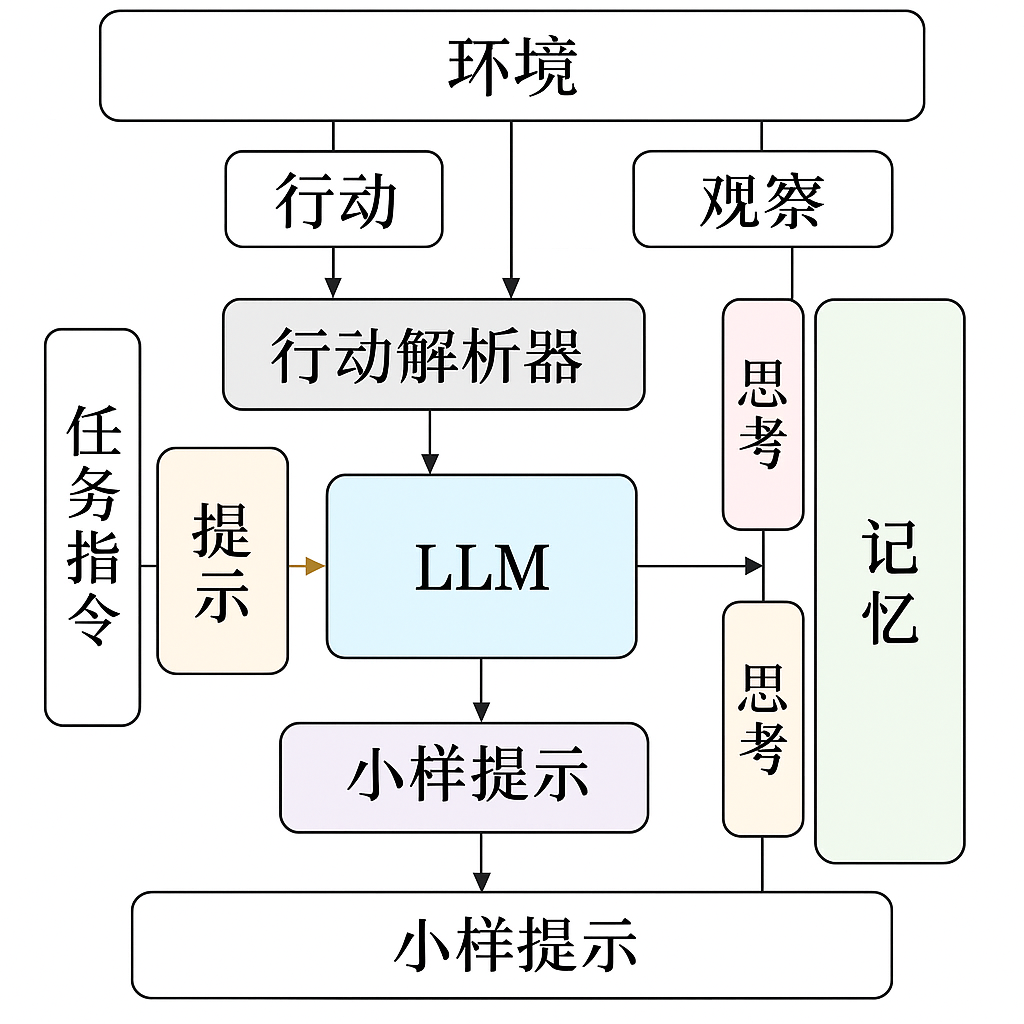
\includegraphics[width=0.35\textwidth]{agent.png}
    \caption{Agent架构示意}
    \label{fig:agent_arch}
\end{figure}

如图\ref{fig:agent_arch}所示,现代Agent架构通常由五个核心组件构成:(1)LLM作为中央决策引擎;(2)工具库提供与外部系统交互的能力;(3)检索增强生成(RAG)—记忆系统存储历史交互和知识;(4)规划系统负责分解复杂任务并制定执行路径;(5)模版提示词提供任务的上下文信息;这种架构使Agent能够执行从简单的信息查询到复杂的多步骤任务,如代码开发、数据分析、自动化办公等多种任务。

然而,随着Agent应用场景的复杂化,传统的计算架构难以满足其高并发、低延迟的处理需求,Serverless架构作为一种新型分布式系统范式正逐渐成为Agent系统的理想基础设施。Serverless架构通过事件驱动和函数即服务(FaaS)模型,实现了计算资源的按需分配与自动扩缩\cite{Baldini2017,jonas2019cloudprogrammingsimplifiedberkeley}。在Agent系统中,每个推理请求、工具调用和状态更新都可被视为独立的函数,由Serverless平台自动调度到最适合的计算节点执行,实现了计算负载的细粒度分解与并行处理。这种架构不仅显著提高了系统的资源利用率,还通过消除冷启动延迟和优化函数间通信,大幅降低了Agent响应时间。特别是对于具有突发流量特性的Agent应用,Serverless架构的弹性伸缩能力可在毫秒级响应需求变化,避免了传统架构中的资源预配过度或不足问题。此外,Serverless的无状态设计与事件溯源模式相结合,为Agent系统提供了天然的容错机制和状态一致性保障,使系统在面对节点故障时仍能保持高可用性和数据完整性。

目前针对Agent性能有两个优化方向,对应Agent中的两个模块,分别是LLM推理和RAG系统。

对于LLM推理这部分优化聚焦在模型架构的基座层面。模型架构优化,通过改进注意力机制等核心算法提升计算效率。例如,FlashAttention-2\cite{dao2023flashattention2fasterattentionbetter}和PagedAttention\cite{10.1145/3600006.3613165}等高效注意力算法,使推理速度提升数倍。更高效的利用硬件资源,利用新一代AI芯片和高速互联技术。并行计算,在多设备间合理分配计算任务。例如,模型并行、张量并行、数据并行等\cite{shoeybi2020megatronlmtrainingmultibillionparameter,10.1145/3458817.3476209,li2020pytorchdistributedexperiencesaccelerating}。内存管理,优化模型参数和中间状态的存储策略。例如KV Cache等\cite{298501}。

对于RAG系统,这部分主要从检索效率和知识管理两个维度展开。向量数据库层面,采用了分层索引结构和异步预加载机制\cite{8594636},将检索延迟降低。同时引入了动态缓存策略,对高频查询结果进行智能缓存。在检索策略上,开发了自适应上下文窗口技术,根据查询复杂度动态调整召回范围,并通过语义相关性重排序提升检索精度\cite{lim2025macragcompressslicescaleup}。此外,通过分布式存储和增量更新机制,实现了知识库的高效扩展和实时更新\cite{li2025eacoragdistributedtieredllm}。

但是,值得注意的是,目前针对Agent性能的两个优化方向的研究未充分利用移动互联网时代积累的宝贵经验——分布式计算。分布式系统在大规模计算场景中具有显著优势:首先,分布式架构支持计算资源的弹性扩展,通过横向扩展节点数量,可以突破单机硬件性能瓶颈,支持异构计算资源的整合,并实现动态资源调配;其次,分布式系统能够实现任务负载的自动均衡,通过智能任务调度、工作窃取机制和数据本地性优化等策略,显著提高资源利用率,减少计算资源的闲置;最后,分布式系统具备较高的可用性,通过多副本冗余、故障检测与自动故障转移等机制,确保系统在部分节点失效时仍能持续提供服务,提升了系统整体的稳定性和可靠性。

然而,将现有的单机Agent系统迁移到分布式环境面临着一系列算法层面的根本性挑战:(1)计算图分割问题——如何将Agent的计算过程表示为有向无环图,并找到最优的图分割方案,使得子图间通信开销最小化,同时保证负载均衡,这本质上是一个NP-Hard问题;(2)状态一致性与并发控制——在分布式环境下维持Agent状态的一致性,需要解决分布式共识算法与异步计算模型之间的矛盾,传统的分布式锁和事务机制在高并发、低延迟的Agent场景下效率低下;(3)动态资源分配与调度——Agent任务的异构性和动态变化特性使得经典的静态资源分配算法难以应用,需要设计能够适应工作负载实时变化的自适应调度算法;(4)容错与恢复机制——分布式Agent系统需要在部分节点失效的情况下保持服务质量,这要求设计高效的检查点与回滚恢复算法,在保证正确性的同时最小化性能开销。这些算法挑战的复杂性远超传统的单机优化问题,使得许多研究者倾向于在单机环境下寻求局部最优解,而非探索分布式环境下的全局最优方案,这也导致了大模型Agent系统在理论上可扩展性受限。

针对这一问题,本文提出了一种低成本、自适应的分布式迁移算法,能够将现有的单机Agent应用自动转换为分布式系统,同时保证了系统的可用性、可靠性、可伸缩性。

\section{本文研究内容及结构安排}

\subsection{本文研究内容}

随着Agent系统日益复杂化和应用场景扩展,其计算需求呈爆发式增长,而现有的单机计算架构已成为性能瓶颈。尽管业界已在LLM推理加速和RAG优化方面取得进展,但这些优化大多聚焦于单一模块的局部性能提升,无法解决Agent系统整体运行效率和规模扩展的根本问题。同时,现有分布式计算技术虽然理论上能够提供解决方案,但对于Agent系统这类具有复杂交互模式和状态依赖关系的应用,缺乏低成本、自动化的迁移方法,开发者仍需大量人力重构代码。这种技术现状与日益增长的Agent应用部署需求之间的矛盾,迫切需要一种能够自动将单机Agent程序转换为分布式系统的技术解决方案。

本文针对Agent系统在分布式环境下的性能优化问题,提出了一种自适应分布式迁移框架,实现单机Agent程序到分布式系统的自动化、透明化转换。
设计了一套量化模块间依赖关系的指标函数体系,包括计算开销度、数据开销度和函数依赖度。
提出了基于依赖指标和资源开销的应用拆分聚类算法,实现模块的最优分布式部署。
实现了完整的分布式框架。分布式编译器自动分析代码结构,生成分布式执行计划。分布式执行器处理任务调度、资源分配和负载均衡。分布式服务器管理节点通信、状态同步和故障恢复。

实验结果表明,本文框架在零代码修改条件下实现了显著的性能提升。在文献调查Agent测试中,将任务执行时间从单机版本的0秒缩短至0秒,提升0\%;在基础性能测试中,比Ray和Dask分别快0\%和0\%;在并行处理测试中,比对比框架快0至0倍;在大数据传输场景下,性能优势更为显著,约为Ray的0倍、Dask的0倍。相比之下,传统框架需要大量代码修改(Ray 0\%,Dask 0\%)才能达到类似性能。本框架为Agent系统提供了低成本、高性能的分布式解决方案,推动了分布式系统的自动化演进。

\subsection{本文结构安排}
本文共分为五个部分,具体结构安排如下:

第一部分为绪论,主要介绍了工作的研究背景及意义,以及研究内容和结构安排。

第二部分为相关工作,主要介绍了大语言模型推理加速、RAG性能优化、分布式计算等方面的相关工作。

第三部分为自适应的单机程序的分布式迁移算法,介绍了本文提出的分布式迁移算法的理论基础。

第四部分为实验测试与分析,主要对本文提出的算法进行了实验验证和分析。

第五部分为展望和结论,对未来的研究方向进行了讨论,并对本文的研究工作进行了总结。

%-----------------------------------------------------------------------------------------

\chapter{相关工作}

本章从大语言模型推理加速、RAG系统性能优化和分布式计算三个维度梳理现有技术,分析它们在解决Agent系统性能瓶颈方面的贡献与局限性。通过对相关工作的系统性分析,本文发现现有技术多聚焦于单个模块的局部优化,如图\ref{fig:accelerate_monolith}所示,缺乏对Agent系统整体性能的全局考量,尤其是缺少将单机Agent应用自动迁移到分布式环境的有效方法。这种研究空白为本文提出的自适应分布式框架奠定了理论基础和应用价值。

\section{大语言模型推理加速}
对Agent计算范式性能优化中,最受到关注的就是大语言模型的推理加速。

Agent系统中,注意力计算是需要重点优化的性能瓶颈,特别是当多个Agent实例并行处理任务时。FlashAttention\cite{NEURIPS2022_67d57c32}通过IO感知计算重构注意力机制,将内存带宽瓶颈显著降低,对分布式Agent系统中的单节点性能有重要提升。特别是,FlashAttention-2\cite{dao2023flashattention2fasterattentionbetter}的改进并行策略与分布式系统资源分配理念高度契合,使其能更好地适应不同计算节点的硬件特性。然而,这些注意力优化仅限于单个LLM的内部计算,无法解决Agent系统中多个异构模块间的协同优化问题,对分布式边缘环境中资源有限的节点支持不足。

Agent系统部署中,内存资源的高效利用对系统可扩展性至关重要。PagedAttention\cite{10.1145/3600006.3613165}借鉴操作系统分页机制,通过非连续内存分配实现了KV Cache的高效管理,这一技术在分布式环境中具有特殊价值:它使单节点能够处理更多并发请求,降低了扩展集群规模的需求。Scissorhands方法\cite{NEURIPS2023_a452a7c6}的动态KV Cache剪枝技术减少了高达70\%的内存占用,在分布式系统中不仅降低了单节点资源消耗,还显著减少了节点间状态同步所需的数据传输量。然而,这些内存优化技术主要针对单个LLM模型设计,在异构分布式Agent系统中缺乏对RAG等其他模块内存需求的整体考量,无法自动根据系统整体负载动态调整不同模块的内存分配策略,限制了在资源受限的边缘分布式环境中的应用效果。

Agent系统中,推测解码技术具有双重价值。减少单节点计算负载的同时,也为系统在节点间的计算分配提供了新的可能性。Chen等人的分阶段推测解码\cite{chen2023acceleratinglargelanguagemodel}技术在分布式环境中可实现小模型和大模型的分节点部署,充分利用边缘节点和中心节点的异构资源。SpecInfer\cite{10.1145/3620666.3651335}的树状推测验证机制在分布式部署中能够自然地将验证任务并行化,显著提高系统吞吐量。然而,这些技术主要聚焦于LLM推理相关的文本生成任务,在分布式Agent中需要扩展以覆盖工具调用、RAG查询等非生成性任务。现有系统无法自动适应这种异构性,需要开发者手动为不同组件定制分布式策略,增加了开发和维护成本。

Agent系统中,操作融合不仅能提高单节点计算效率,还能优化节点间计算与通信的协同模式。Salmani和Soloveychik的操作融合技术\cite{salmani2025llminferenceaccelerationefficient}通过重组Softmax和LayerNorm等操作,将其计算与线性层并行执行,在分布式环境中能够减少计算节点之间的必要同步点,降低通信开销并减少约20\%的端到端延迟。然而,这种操作融合仅针对LLM内部计算进行优化,不能应用于Agent系统中更高级别的模块间融合,如RAG检索与GPT推理的跨模块融合。在异构分布式环境中,缺乏一种自适应的方法来统一优化不同硬件节点上的计算操作,这大大限制了整体系统的性能提升。

Agent系统中,量化技术不仅能降低单节点计算负载,还能显著减少节点间通信开销,为Agent系统分布式部署提供关键支持。SmoothQuant\cite{pmlr-v202-xiao23c}作为一种无需额外训练的后训练量化(PTQ)方法,实现了大语言模型的8位权重、8位激活(W8A8)量化,将模型大小压缩至2倍,为分布式部署中的模型分片和负载均衡创造了条件。在分布式环境中,量化带来的内存减少和计算加速允许在同一硬件资源上部署更多Agent实例,提高了系统整体吞吐量。特别是,量化技术减少了节点间传输的数据量,缓解了分布式系统中的网络带宽瓶颈。然而,这些单一模型的量化方法主要聚焦于降低单节点资源消耗,对Agent系统中LLM与RAG等模块之间的分布式协同考虑不足,无法自动根据不同节点的资源特性进行自适应量化与负载分配,限制了其在异构分布式环境中的效益。

这些技术从不同角度优化了大语言模型的推理过程,为Agent计算范式提供了坚实基础。但是,这些技术的优化都只聚焦了大语言模型本身,对Agent计算范式中的其他组件,如RAG系统,未进行系统研究,不能对整个Agent系统的性能进行优化。

\begin{figure}[h]
    \centering
    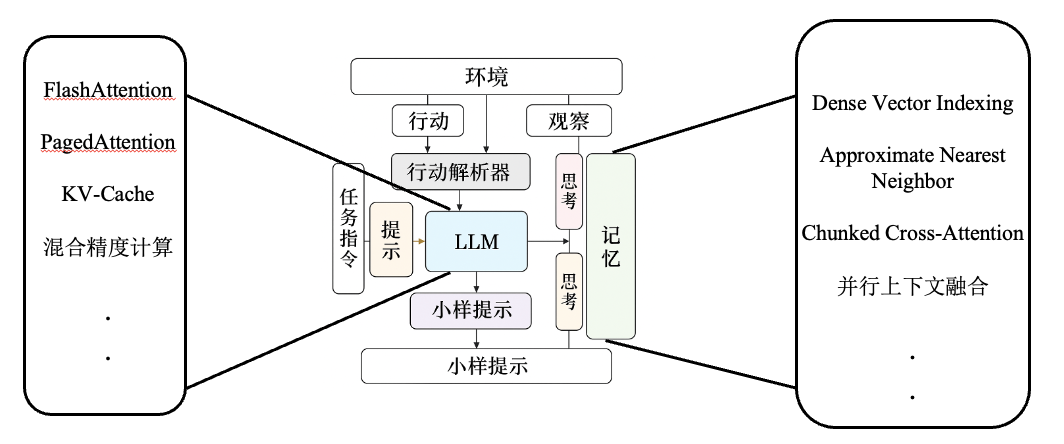
\includegraphics[width=\textwidth]{agent_intra.png}
    \caption{Agent系统只关注单一模块的加速优化}
    \label{fig:accelerate_monolith}
\end{figure}

\section{RAG性能优化}
RAG是Agent系统的核心组件之一,为Agent提供外部知识获取能力。在Agent架构中,RAG负责从知识库检索相关信息,增强大模型的上下文理解和推理能力,使Agent能够基于最新、准确的信息做出决策。高效的RAG系统直接影响Agent的响应速度和决策质量,因此RAG性能优化对整个Agent系统的性能至关重要。

缓存中间计算结果是提高RAG系统效率的有效方法。Kwon等人\cite{jin2024ragcacheefficientknowledgecaching}提出了RAGCache,一种多级动态缓存系统,专为RAG优化设计。该系统将检索文档的中间状态(key-value张量)存储在知识树结构中,采用前缀感知的贪婪双大小频率(PGDSF)替换策略管理缓存。实验表明,与传统方法相比,RAGCache可将首个token生成时间(TTFT)减少高达4倍,吞吐量提高最多2.1倍。类似地,SGLang系统也采用了缓存技术,但RAGCache通过更有效的缓存策略进一步提升了性能。

检索深度对RAG系统性能有显著影响。Hall等人\cite{stuhlmann2025efficientreproduciblebiomedicalquestion}在生物医学问答系统中研究了检索深度与系统效率的关系。他们发现,在使用BM25和MedCPT的混合检索策略时,检索50篇文档后进行重排序能在准确性(0.90)、召回率(0.90)和响应时间(1.91秒)之间取得最佳平衡。该研究表明,超过特定阈值的检索深度不仅增加计算成本,还可能导致性能下降,这为RAG系统设计提供了重要参考。

并行计算是减少RAG系统端到端延迟的关键技术。Kwon等人\cite{jin2024ragcacheefficientknowledgecaching}提出的动态推测流水线技术通过重叠知识检索和LLM推理过程,显著减少了系统响应时间。Zhang等人\cite{295471}在向量数据库优化方面的工作表明,高效的检索算法能将检索时间控制在毫秒级别,从而为计算并行化创造条件。此外,缓存感知的请求调度策略也被证明能有效提高系统的整体吞吐量\cite{zhang2022bufferpoolawarequery}。

向量数据库作为RAG系统检索环节的核心,其性能直接影响整体响应速度。Johnson等人\cite{10.1109/TPAMI.2018.2889473}提出的HNSW(分层可导航小世界图)算法通过构建多层近似图结构,在数十亿级向量库上实现了亚线性时间复杂度的检索。Facebook AI研究院开发的Faiss库\cite{douze2025faisslibrary}引入了产品量化和倒排索引技术,显著降低了内存占用并加速了向量检索。最近,Zhang等人\cite{NEURIPS2019_09853c7f}提出的DiskANN算法针对SSD存储优化,解决了大规模向量数据库的内存限制问题,同时保持了毫秒级的查询延迟。此外,Pinecone等商业系统通过混合索引结构和分布式部署,进一步提高了向量数据库在云环境中的可扩展性和吞吐量。这些优化技术使向量检索时间从秒级降至毫秒级,为RAG系统的实时响应奠定了基础。

目前,RAG系统优化仍聚焦于检索模块本身,这种单一模块的优化方法虽然取得了一定成效,但缺乏对Agent系统整体架构的全局考量。这种局部优化策略无法解决跨模块交互产生的性能瓶颈,也忽略了系统层面的资源调度与并行处理机会,导致整体加速效果有限。从系统工程角度看,真正有效的性能提升需要综合考虑所有模块的协同工作模式,而非孤立地优化单个组件。


\section{分布式计算}

随着Agent系统日益复杂化,大规模部署面临严峻的性能挑战。Agent系统的异构特性(包含LLM推理、RAG检索、工具调用等多个组件)和动态工作负载需要高度灵活的计算架构支持。分布式计算技术凭借其弹性资源管理、并行处理能力和故障容错机制,为Agent系统提供了理想的底层架构支持。然而,传统分布式系统往往关注大规模数据处理而非交互式应用场景,使其难以直接应用于具有严格延迟要求的Agent系统。本节综述了分布式计算领域的相关工作,包括无服务器计算、分布式计算引擎和自动并行化技术,并分析了这些技术在Agent系统分布式迁移方面的应用潜力与局限性。


无服务器计算作为一种新兴的云计算范式,彻底改变了应用程序的开发和部署方式。Berkeley团队的开创性研究\cite{jonas2019cloudprogrammingsimplifiedberkeley}详细分析了无服务器计算的优势与局限性,并指出了其面临的技术挑战。该团队随后提出了对无服务器计算未来发展的展望,为这一领域奠定了理论基础。在AWS开发的Firecracker\cite{246288}中,轻量级虚拟化技术显著降低了函数冷启动开销,而SOCK\cite{216031}和SAND\cite{215935}则通过优化容器设计和调度提高了执行效率。Catalyzer\cite{10.1145/3373376.3378512}的无初始化启动技术将冷启动时间降至亚毫秒级,而FaasCache\cite{10.1145/3445814.3446757}通过高效缓存策略延长了函数实例生命周期。然而,这些无服务器计算技术主要聚焦于单一函数的优化,缺乏对复杂应用自动分布式迁移的系统支持。特别是对于Agent系统,其异构组件(如LLM推理和RAG模块)之间的复杂交互模式和状态依赖关系,使得现有的计算模式无法直接在无服务器框架下高效处理,仍然需要大量人力修改程序。本文提出的分布式迁移算法借鉴了无服务器计算的资源按需分配理念,同时通过深度依赖分析和自适应图分割技术,解决了传统无服务器架构在处理复杂Agent应用时的局限性。

在大规模数据处理方面,MapReduce\cite{10.1145/1327452.1327492}首先提出了简单而强大的编程模型,通过键值对映射与归约操作实现分布式计算。随后,Apache Spark通过弹性分布式数据集\cite{10.5555/2228298.2228301}的抽象,实现了内存计算和数据复用,大幅提高了迭代计算性能。Apache Flink\cite{10.14778/3137765.3137777}则引入了流式处理范式和状态管理机制,支持低延迟、高吞吐的流处理。近年来,Ray\cite{10.5555/3291168.3291210}提出了统一任务并行和Actor模型的分布式框架,特别适合AI工作负载,其动态执行图和分布式调度器能够有效处理异构计算任务。Dask\cite{rocklin2015dask}则为Python生态提供了可扩展的并行计算解决方案,支持类NumPy、Pandas的并行API。这些分布式计算引擎虽然强大,但大多要求开发者显式定义并行策略并手动编写注释代码,缺乏针对已有单机Agent系统的自动迁移能力,且难以处理Agent系统中复杂的状态依赖关系和函数调用模式。

自动并行化技术的理论基础已通过数十年的研究得到严谨确立。Allen和Kennedy\cite{10.5555/502981}的开创性工作通过依赖分析和循环变换技术奠定了基础,而现代框架如Pluto、Polly和PPCG等展示了静态代码分析在提取并行性方面的成熟应用。在提高编程生产力方面,Stanford的Gluon\cite{gluon2017}框架通过数据和计算分离策略,使算法专家能够关注算法逻辑而非分布式实现细节。MIT的Swift\cite{10.1145/2442516.2442559}系统提供了数据流编程模型,能够自动提取任务级并行性并处理依赖关系。Google的MLIR\cite{lattner2020mlircompilerinfrastructureend}编译器基础设施通过多级中间表示,能够自动识别并优化并行模式。AutoParallel\cite{ramoncortes2018autoparallelpythonmoduleautomatic}项目将静态分析与运行时调度相结合,实现了Python程序的自动并行化。值得注意的是,Ban首次提出了透明分布式化的概念\cite{10.5555/256664.256760},通过运行时拦截实现了对现有Python应用的无侵入分布式迁移,但其静态依赖分析能力有限,难以处理动态特性丰富的Agent系统。这些自动并行化系统大多聚焦于特定领域或编程模型,无法有效处理Agent系统中多样的组件交互模式和复杂状态依赖,特别是在面对RAG和LLM等组件结合时的动态性能特征。本文的工作从这些经典自动并行化理论中汲取关键洞见,并将其应用于通用程序的自动分布式部署,特别是解决了传统自动并行化理论到现代分布式计算之间的理论鸿沟。

\begin{figure}[htbp]
    \centering
    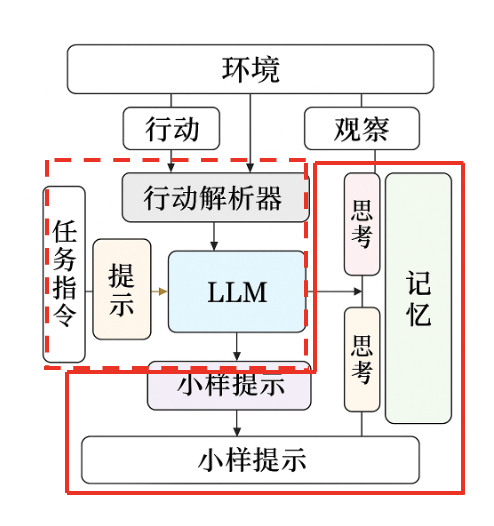
\includegraphics[width=0.4\textwidth]{agent_extra.png}
    \caption{Agent系统的分布式加速优化}
    \label{fig:accelerate_distributed}
\end{figure}

上述工作为分布式计算提供了丰富的技术基础,但面对本文关注的Agent系统分布式迁移问题,这些方法仍存在明显局限性:首先,它们缺乏针对Agent特定组件(如LLM推理和RAG系统)的深度优化;其次,现有分布式编程框架要么抽象层次太低,编程负担大。要么需要重新编写程序手动调优设计;最后,传统并行计算的方法,针对特定编程场景的框架与Agent系统的交互型应用场景存在不匹配。本文提出的自适应分布式迁移算法正是针对这些挑战,通过精细化的依赖分析、自适应图分割和透明拦截技术,实现了对单机Agent系统的高效分布式迁移,如图\ref{fig:accelerate_distributed}所示,同时平衡了系统吞吐量和响应延迟。

%=========================================================================================
